\documentclass[10pt,a4paper]{article}
\usepackage[latin1]{inputenc}
\usepackage[english]{babel}
\usepackage{amsmath}
\usepackage{amsfonts}
\usepackage{amssymb}
\usepackage{graphicx}
\usepackage{fancyhdr}
\usepackage{lastpage}
\usepackage{multirow}

%Include and define  c code
\usepackage{listings}
\usepackage{color}
\usepackage{textcomp}
\definecolor{listinggray}{gray}{0.9}
\definecolor{lbcolor}{rgb}{0.9,0.9,0.9}
\lstset{
	language=C,
	keywordstyle=\bfseries\ttfamily\color[rgb]{0,0,1},
	identifierstyle=\ttfamily,
	commentstyle=\color[rgb]{0.133,0.545,0.133},
	stringstyle=\ttfamily\color[rgb]{0.627,0.126,0.941},
	showstringspaces=false,
	basicstyle=\small,
	numberstyle=\footnotesize,
	numbers=left,
	stepnumber=1,
	numbersep=10pt,
	tabsize=2,
	breaklines=true,
	prebreak = \raisebox{0ex}[0ex][0ex]{\ensuremath{\hookleftarrow}},
	breakatwhitespace=false,
	aboveskip={1.5\baselineskip},
  columns=fixed,
  upquote=true,
  extendedchars=true,
 frame=single,
 backgroundcolor=\color{lbcolor},
}

\oddsidemargin  -0.5cm
\evensidemargin 0.0cm
\textwidth      17.25cm
\headheight     1.0cm
\headsep		0.7cm
\topmargin      -0.5cm
\textheight		22.0cm

\pagestyle{fancy}
\lhead{Exercise 5}
\chead{EEMB1}
\rhead{\thepage\ of \pageref{LastPage}}
\lfoot{Theis Christensen\\Paulo Fontes\\Dennis Madsen}
\cfoot{Team3}
\rfoot{\today}
\renewcommand{\headrulewidth}{0.4pt}
\renewcommand{\footrulewidth}{0.4pt}
\begin{document}
\part*{EMB 2010 Team3 Exercise2}
\section{Some setup}
This exercise is about making one big loop out of UART 0, 1, 2.
It is done by sending a character from the pc into the first UART, UART0 which reads the character and sends it to
UART2, the UART2 reads the input and sends the character back to the pc. When the character is sent further on in the system
one is added to the value.\\
Ex. The PC sends the character 'a'. UART0 receives this value, adds one to it ('b') and sends it further on in the loop. 
UART2 receives the character, adds one to it and returns it to the PC, where the value 'c' appears on the screen.\\
Unfortunately we could not get UART1 to work on the 32-bit board we have, otherwise it would also have been part of the loop.
From the 'LPC2489 Users Guide':
\\ \textit{ Full modem RS232 on UART1 (cannot be used on 32-bit data bus cpu boards, 
but RxD2/TxD2 can alternatively be connected to the RS232 interface)}

\begin{figure}[h!]		%Remember to put the h!, to not fuck the sections.
 \begin{centering}
  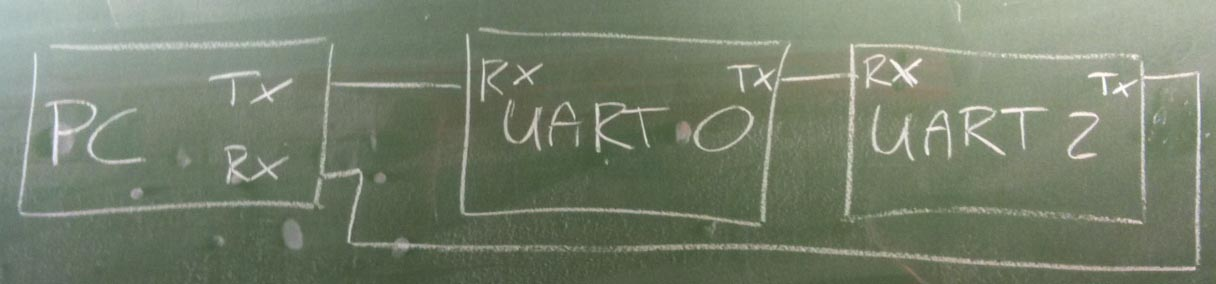
\includegraphics[width=0.8\textwidth]{setupbb.jpg}
   \caption{How it is meant that the hardware should be putted together. }
 \end{centering}
\end{figure}

\begin{figure}[h!]		%Remember to put the h!, to not fuck the sections.
 \begin{centering}
  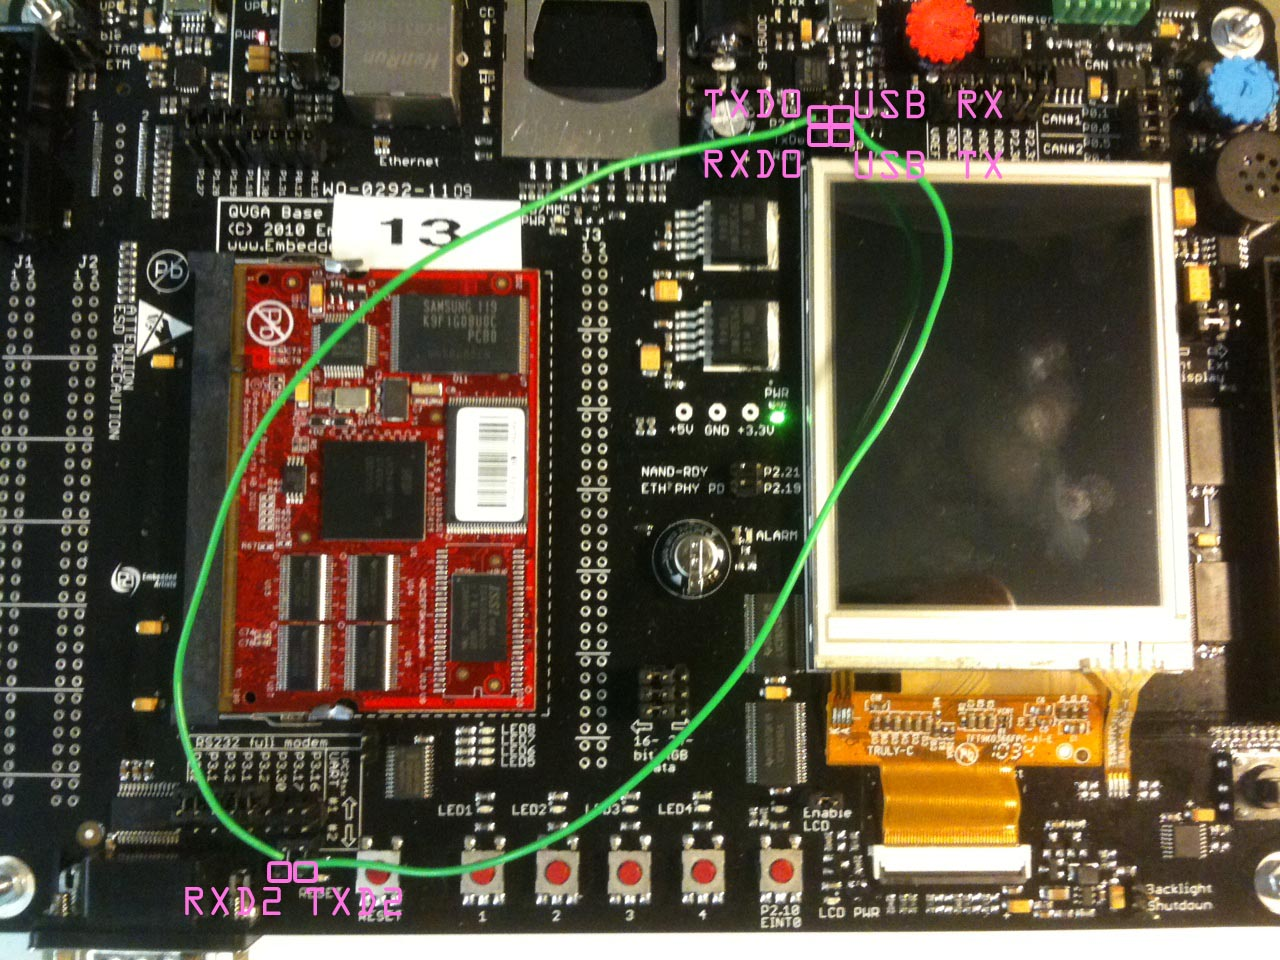
\includegraphics[width=0.72\textwidth]{setup.jpg}
   \caption{How the hardware implementation is realised.}
 \end{centering}
\end{figure}
\newpage
\begin{figure}[h!]		%Remember to put the h!, to not fuck the sections.
 \begin{centering}
  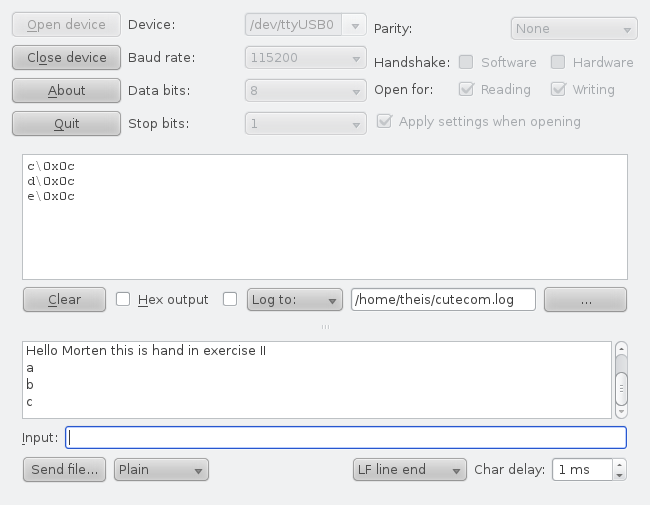
\includegraphics[width=0.8\textwidth]{uart.png}
   \caption{What is sent and what is received. Note: the "system" is also tried with other baud rate setups and works fine.}
 \end{centering}
\end{figure}

\section{Some code}
In the start of the code some peripherals are set up in the lowLevelInit function, such as power enable registers, clock speed etc.
'initUart' is called twice to set up both UART0 and UART2.\\
In the 'system loop' the program simply waits for an input from the PC, sends the character to the UART2 (HW linked).
The UART2 reads the character and sends it back to the pc.

\begin{figure}[h!]		%Remember to put the h!, to not fuck the sections.
 \begin{centering}
  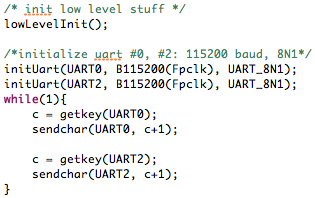
\includegraphics[width=0.42\textwidth]{main.png}
   \caption{The main loop and initial setup.}
 \end{centering}
\end{figure}

\newpage
The initialization is only changed a little compared to the given example. Simply a switch-case is made, to setup only the selected UART. 

\begin{figure}[h!]		%Remember to put the h!, to not fuck the sections.
 \begin{centering}
  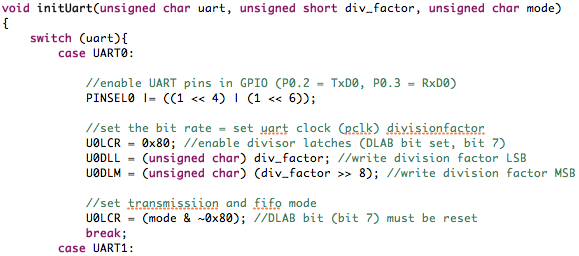
\includegraphics[width=0.7\textwidth]{inituart.png}
   \caption{Initialisation of UARTx.}
 \end{centering}
\end{figure}

The send and receive functions are also just expanded to send and receive characters to/from the selected UART port (switch-cases are used).

\begin{figure}[h!]		%Remember to put the h!, to not fuck the sections.
 \begin{centering}
  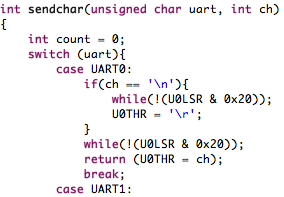
\includegraphics[width=0.35\textwidth]{senduart.png}
   \caption{Send a character to UARTx.}
 \end{centering}
\end{figure}

\begin{figure}[h!]		%Remember to put the h!, to not fuck the sections.
 \begin{centering}
  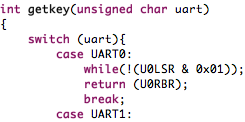
\includegraphics[width=0.3\textwidth]{recieveuart.png}
   \caption{Read a character from UARTx.}
 \end{centering}
\end{figure}

The power (PCUART) is by default enabled for channel 0 and 1, but disabled for channel 2 and 3. Therefore all of these is enabled in the framework.c file
(the lowLevelInit function).

\begin{figure}[h!]		%Remember to put the h!, to not fuck the sections.
 \begin{centering}
  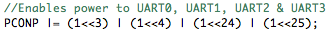
\includegraphics[width=0.37\textwidth]{powerenable.png}
   \caption{Power on all UART modules.}
 \end{centering}
\end{figure}

\end{document}
